\normallinespacing

\chapter{The Reinforcement Learning Paradigm}

Reinforcement Learning (RL) is a sub-field of machine learning wherein an agent learns to take optimal decision in an unknown environment by trial and error.
RL differs from the other branches of machine learning -- namely supervised learning and unsupervised learning.
Supervised learning involves learning from labeled data whereas unsupervised learning involves finding the underlying structure of unlabeled data.
RL involves an agent actively exploring an interactive environment sequentially and
performing actions to maximize a "reward" metric over a number of steps.

\begin{figure}[!htbp]
    \centering
    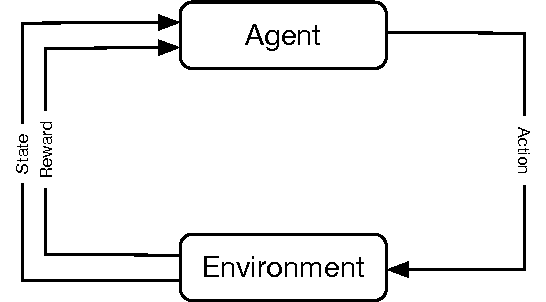
\includegraphics{rl/rl_scheme.pdf}
    \caption{The basic reinforcement learning scheme.}
    \label{fig:rl_scheme}
\end{figure}

In the RL paradigm, at each time step, an agent interacts with the environment by choosing an action based on its present state using a learned policy $\pi$.
Then the agent transitions onto a new state as dictated by the dynamics of the environment.
It receives a scalar feedback, a reward, pertaining to its previous action in the process.
This chapter serves as a brief introduction to the reinforcement learning paradigm and introduces its various components that will be used throughout the manuscript.

\section{Markov Decision Processes}

A typical model of an environment in RL task is represented as a Markov Decision Processes (MDP).
To achieve a goal in a MDP, the learning agent has to learn the parameter of the MDP and take optimal decisions based on these learned parameters.
Formally, an MDP, $M$, in the undiscounted reward setting, is defined as the quintuple $M = \langle \mathcal{S}, \mathcal{A}, \mathcal{R}, \mathcal{P} \rangle$, where the various components are defined as follows:

\subsection{State Space}

A state is a representation of the agent's environment.
The state space is defined as the set of states that the MDP can be in , it is denoted by $\mathcal{S}$.

\subsection{Action Space}

It is the set of possible moves available to the agent at any state, denoted by the set $\mathcal{A}$.
Taking an action may cause the agent to transition from one state to another.

\subsection{Reward}

It is a scalar feedback received from the environment as a consequence of the agent's action.
A characteristic of reinforcement learning is the delayed rewards.
It means that the consequence of an action is not immediate, its effect is observed in the future.

\subsection{Transition Probabilities}

$\mathcal{P}$ is a transition probability kernel.
$\mathcal{P}(s^\prime \mid s, a)$ denotes the probability of transitioning from state $s$ to another state $s^\prime$ after an action $a$ is executed.

\section{Action Policy}

Policy $\pi$ characterizes the behavior of the learning agent in a state $s$. 
It qualifies the action(s) that the agent will undertake in a particular state $s$.

A policy can be \textbf{stochastic}, it induces a probability distribution over the set of actions $\mathcal{A}$ for a given state s.

A policy may be \textbf{deterministic}, it maps each state from the set of states $\mathcal{S}$ to a single action from the set of actions $\mathcal{A}$.

A policy may \textbf{depend} on the sequence of all previous states, i.e. the \textbf{history}, that the learner has visited. 

A policy may also be \textbf{Markov} (where that current state is a sufficient statistic of the previous states), it only depends on the current state $s$ that the learner is in. 
A Markov policy is also a \textbf{stationary} in nature.

\section{Objective}

The objective in the RL problem is to maximize an intrinsic reward metric subject to the dynamics of the environment governed by its underlying MDP.
Settings such as discounted sum of rewards, cumulative sum of rewards exist in reinforcement learning paradigm but we will be focusing on the average reward setting in this work.


\section{Gain}
Starting from state $s$ following the policy $\pi$, formally the objective to maximize in the average reward setting is defined as

\begin{equation}
    \label{eqn:gain}
    \lim_{T \to \infty} \mathbb{E}\left[\frac{1}{T} \sum_{t=0}^{T} R_t \mid S_0 = s\right]
\end{equation}

where, $T$ is the time horizon and $R_t$ is the reward is the reward realized in state $S_t$ when $a_t$ is executed where $a_t$ is chosen according to the action policy $\pi$.

Equation \ref{eqn:gain} formally defines the \textbf{gain} following an action policy $\pi$.

\subsection*{Gain Optimality}

The maximal (optimal) gain ($\rho^*$) of an MDP starting at state $s$ in the infinite-horizon setting with average rewards is formally defined as

\begin{equation}
    \label{eqn:gain_opt}
    \rho^*(s) = \max_\pi \mathbb{E}\left[\lim_{T \to \infty} \frac{1}{T} \sum_{t=0}^{T} R_t \mid S_0 = s\right]
\end{equation}
where, $R_t$ is the reward is the reward realized in state $S_t$ when $a_t$ is executed where $a_t$ is chosen according to the gain-optimal action policy $\pi^*$.

\section{Bias}

The bias of a policy $\pi$ is the measure of the total deviation of the reward from the asymptotic average reward.
It is formally defined as

\begin{equation}
    \label{eqn:bias}
    h^\pi(s) = \mathbb{E}^\pi\left[\lim_{T \to \infty} \sum_{t=0}^{T} (R_t - \rho^\pi(S_t)) \mid S_0 = s\right]
\end{equation}

where, $R_t$ is the reward realized in state $S_t$ when $a_t$ is executed where $a_t$ is chosen according to the action policy $\pi$.

\subsection*{Bias Optimality}

A policy $\pi^*$ is bias-optimal if the policy $\pi^*$ gain-optimal and also maximizes the bias values such that $h^{\pi^*} (s) > h^\pi(s)$ for all states $s \in \mathcal{S}$ and policies $\pi$.

\section{Value Function}

The value of a state $s$ under a policy $\pi$, $v^\pi(s)$, is defined as the reward that can be accumulated starting from that state and taking actions according to the policy $\pi$. 
In the average reward setting, the value of a state is measured as the accumulated sum of the average adjusted rewards as the undiscounted sum of rewards may be unbounded.
In other words, the value of state $s$ is equivalent to the bias of that state $s$.

\section{MDP Classes}

MDPs can be classified into various categories based on its transition probability and the policy being executed. They are briefly described below.

\subsection{Communicating States}

Two states $s_1$ and $s_2$ in an MDP are said to be communicating under a policy $\pi$ if there is a non-zero probability of reaching each state from the other in zero or more state transitions.

\subsection{Recurrent States}

A state $s$ is recurrent if there is a non-zero probability of returning to the same state under a policy $\pi$ in zero or more state transitions.
In other words, the probability of eventually returning to state $s$ is one.

\subsection{Ergodic Class of States}

A subset of states are said to belong to an ergodic class if they are recurrent, communicate with each other and do not communicate with any states outside the class.
A Markov chain is irreducible if $\mathcal{S}$, the set of all states, forms an ergodic class.

\subsection{Ergodic MDP}

An MDP is ergodic if the transition matrix corresponding to every policy has a single recurrent class of states.

\subsection{Communicating MDP}

An MDP is communicating if each pair of states communicate with each other under some stationary policy $\pi$.

\section{Bellman Optimality Equations}

Assuming communicating MDPs, Puterman \cite{puterman_chapter_1990} showed that for the optimal gain policy, the optimal average infinite horizon reward does not depend on the starting state. In other words, $\rho^*(s) = \rho^*$.

For a communicating MDP, let $h^*$ be the bias of the optimal policy $\pi^* = \arg \max_\pi \rho^\pi$ and $\rho^*$ be the optimal gain. 
Then, the Bellman optimality equations state that the optimal gain $\rho^* = \rho$ is a feasible solution of the equations below 

\begin{equation}
    \rho^* + h^*(s) = \max_a \left( R(s, a) + \sum_{s^\prime} \mathcal{P}(s^\prime \mid s, a) h^*(s) \right) \quad \forall s \in \mathcal{S}
\end{equation}

where, $R(s,a) = \mathbb{E}_{s^\prime \sim \mathcal{P}(\cdot \mid s, a)}\left[ R(s, a, s^\prime) \right]$ is the expected reward realized at state $s$ taking action $a$.

\section{Value Iteration}

From the recursive definition of the Bellman optimality equation, an iterative algorithm can be formulated. 
This is motivated by the fact that using dynamic programming approaches is infeasible for computationally large state, action spaces and large or infinite time horizons.
One such algorithm is the value iteration algorithm. The value iteration algorithm for the average reward scenario as proposed by Hordijk and Tijms \cite{hordijk_modified_1975} is described in Algorithm \ref{alg:vi}.

\begin{algorithm}[!htbp]
    \SetKwInOut{KwInit}{Initialize}
    \SetKwInOut{KwOut}{Output}
    
    \KwInit{Set $v_0 = 0, v_{-1} = -\infty, k = 0$}
    
    \BlankLine
    \While{$\max_s(v_k(s) - v_{k-1}(s)) - \min_s(v_k(s) - v_{k-1}(s)) > \epsilon$}{
    \BlankLine
    For all $s \in \mathcal{S}$, update
    
    $\quad v_{k+1}(s) = \max_a \left(R(s, a) + \sum_{s^\prime} \mathcal{P}(s^\prime \mid s, a) v_k(s^\prime) \right) - v_k(s)$
    
    Set $k = k + 1$ 
    \BlankLine
    }
    \BlankLine
    \KwOut{$v_{k + 1}$}
    \caption{Pseudocode for Value Iteration}\label{alg:vi}
\end{algorithm}

Value iteration converges to an optimal policy in a finite number of iterations \cite{puterman_chapter_1990} if there exists a state $s$ that is reachable from all other states under all stationary policies.

The policy computed after value iteration is greedy with respect to the computed values.
Formally it can be written as

\begin{equation}
    \pi(s) \in \arg\max_{a \in \mathcal{A}} \left( R(s, a) + \sum_{s^\prime}{\mathcal{P}(s^\prime \mid s, a)} v(s) \right) \quad \forall s \in \mathcal{S}
\end{equation}

where, $v(s)$ is the value computed by value iteration.

\section{Reinforcement Learning in MDPs}

An agent interacts with an environment characterised by the MDP $M$ where $M = \langle \mathcal{S}, \mathcal{A}, \mathcal{R}, \mathcal{P} \rangle$.
The agent has knowledge of set of states $\mathcal{S}$ and the set of actions $\mathcal{A}$ but is unaware of the state transition probabilities and the associated rewards.
The agent gains experience about the environment by interaction in a single trajectory of actions.
The objective of the agent is to maximize the accumulated rewards by exploiting information gathered through the course of its interaction with the environment.

\section{Regret}

The learning performance of an agent is quantified with the measure of its regret.
Regret of an algorithm $\mathbb{A}$ is defined as the difference in the cumulative reward by the optimal policy with that of the algorithm $\mathbb{A}$.
From Definition 3 of Talebi and Maillard \cite{talebi_variance-aware_2018}, regret can be formally is defined as

\begin{equation}
    \label{eqn:regret}
    \text{Regret}(\mathbb{A}, T) = \sum_{t = 0}^T r^*_t - \sum_{t = 0}^T r_t 
\end{equation}

where, $r^*_t = R(S^*_t, \pi^*(S^*_t))$ is the reward obtained at state $S^*_t$ by executing an action according to the optimal policy $\pi^*$ and $r_t$ is the reward obtained at state $S_t$ by executing an action chosen by the algorithm $\mathbb{A}$ at time-step $t$.
The trajectory generated by following the optimal policy $\pi^*$ differs from the trajectory generated by the algorithm $\mathbb{A}$, in other words, $S^*_t$ may be different from $S_t$.
The objective of the agent can be alternatively defined as minimization of the accumulated regret.

Using the Azuma-Hoeffding's inequality, the accumulated regret by following the optimal policy can be upper bounded with probability $1 - \delta$ as

\begin{equation*}
    \sum_{t = 0}^T r^*_t \le T g^* + \mathcal{O}(\sqrt{\log(2/\delta)}) 
\end{equation*}

where, $g^*$ is the optimal gain. Thus, Equation \ref{eqn:regret} can be rewritten as

\begin{equation*}
    \text{Regret}(\mathbb{A}, T) \le T g^* - \sum_{t = 0}^T r_t + \mathcal{O}(\sqrt{\log(2/\delta)})
\end{equation*}

or, alternately, regret can be defined as

\begin{equation}
    \label{eqn:theogregret}
    \Delta(\mathbb{A}, T) =  T g^* - \sum_{t = 0}^T r_t
\end{equation}

minimizing which is asymptotically equivalent to finding a gain-optimal policy.

% Links - 
% https://ieor8100.github.io/rl/docs/Lecture%201%20-MDP.pdf
% http://proceedings.mlr.press/v119/bourel20a/bourel20a.pdf
% https://arxiv.org/pdf/2009.04575.pdf

